\documentclass{article}
\usepackage[utf8]{inputenc}
\usepackage{geometry}
\usepackage{amsmath}
\usepackage{physics}
\usepackage{graphicx}
\usepackage{textcomp}
\usepackage{hyperref}
\geometry{legalpaper, portrait, margin = 0.5in}
\rmfamily

\title{AMS 261 HW9}
\author{David S. Li (SBUID: 110328771)}
\date{October 31, 2018}

\begin{document}

\maketitle

\par\noindent\large Outside resources used: \url{https://www.youtube.com/watch?v=dD03-YJJUfM}
\renewcommand{\thefootnote}{\roman{footnote}}

\section{14.3.4 - Sketch the region of integration represented by the double integral $\int_{0}^{2\pi}\int_{3}^{6}f(r, \theta)drd\theta$}

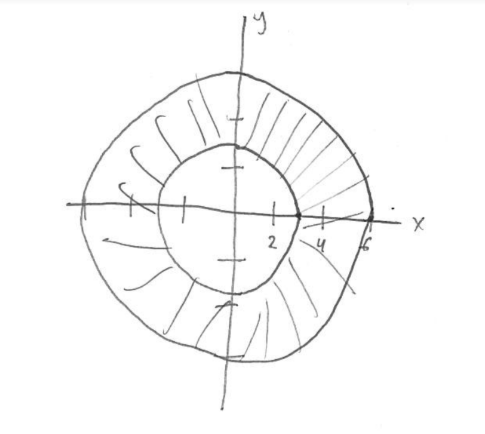
\includegraphics[]{Problem1.PNG}\centering

\raggedright

\section{14.4.48 - The center of mass of the lamina of constant density shown in the figure is $(2, \frac{8}{5})$.  Make a conjecture about how the center of mass $(\Bar{x}, \Bar{y})$ changes for each given nonconstant density $\rho(\Bar{x}, \Bar{y})$.  Explain. (Make your conjecture \textit{without} performing any calculations)}
\subsection{(a) $\rho(x, y) = ky$}
\par\noindent\large Any changes in $x$ will not affect the center of mass, while any changes of $y$ will be proportional to any change incurred on the center of mass. (i.e., if $y$ increases, $\rho$ will increase)

\subsection{(b) $\rho(x, y) = k\abs{2 - x}$}
\par\noindent\large Any changes in $y$ will not affect the center of mass, while $\rho$ will depend on the absolute value of $2 - x$ (you would get a cone shaped graph for the function of $\rho$)

\subsection{(c) $\rho(x, y) = kxy$}
\par\noindent\large $\rho$ is proportional to the \textit{product} of $xy$. (The \textit{product} has to change overall for any change in $\rho$)

\subsection{(d) $\rho(x, y) = k(4 - x)(4 - y)$}
\par\noindent\large $\rho$ is proportional to the \textit{product} of $(4 - x)(4 - y)$. (Again, the \textit{product} has to change overall for any change of $\rho$)

\section{14.6.2 - Why is it beneficial to be able to change the order or integration for a triple integral?}
\par\noindent\large Because we can potentially be integrating over a wide variety of surfaces, with their $x$, $y$, and $z$ dimensions represented as potentially crazy equations, it can sometimes be beneficial to change the order of integration to potentially simplify the work we have to do.  For example, if integrating in the order $dzdydx$ potentially gave us a crazy complicated bounds expression(s) to put in our integral and evaluate, but another order  like $dzdxdy$ had a bounds expression(s) that wasn't so complicated, that would be much more preferable for integrating over as compared to integrating using the traditional $dzdydx$.

\section{14.7.42 - Convert the integral from rectangular coordinates to both cylindrical and spherical coordinates, and evaluate the simplest iterated integral: $\int_{0}^{2}\int_{0}^{\sqrt{4 - x^{2}}}\int_{0}^{\sqrt{16 - x^{2} - y^{2}}}\sqrt{x^{2} + y^{2}} dzdydx$}

\par\noindent\large Based on the above information, we have bounds $0 \leq x \leq 2$, $0 \leq y \leq \sqrt{4 - x^{2}}$, and $0 \leq z \leq \sqrt{16 - x^{2} - y^{2}}$ in rectangular form.

\subsection{Rectangular\textrightarrow Cylindrical}
\par\noindent\large  We can rearrange $\sqrt{16 - x^{2} - y^{2}} = z \rightarrow z^{2} = 16 - x^{2} - y^{2}$ and $y = \sqrt{4 - x^{2}} \rightarrow x^{2} + y^{2} = 4$.  Converting the equations to polar form gives us $z^{2} = 16 - r^{2}$ and $r^{2} = 4$.  Taking the square roots of each of the functions accordingly, we get $z = \sqrt{16 - r^{2}}$ and $r = 2$ (discarding any negative values because we are dealing with distance).\vspace{0.25cm}

\par\noindent The iterated triple integral in cylindrical form is:
\par\noindent\Large $\int\int_{Q}\int f(x, y, z)dV = \int_{\theta_{1}}^{\theta_{2}}\int_{g_{1}(\theta)}^{g_{2}(\theta)}\int_{h_{1}(rcos(\theta), rsin(\theta))}^{h_{2}(rcos(\theta), rsin(\theta))}f(rcos(\theta), rsin(\theta))r dzdrd\theta$

\par\noindent\large Our bounds, converted are, starting from the inner-most integral: $0 \leq z \leq \sqrt{16 - r^{2}}$, $0 \leq r \leq 4$, $0 \leq \theta \leq \frac{\pi}{2}$, and $\sqrt{x^{2} + y^{2}} = r$ in polar/cylindrical coordinates.\vspace{0.25cm}

\par\noindent\Large This gives us the iterated integral: $\int_{0}^{\frac{\pi}{2}}\int_{0}^{2}\int_{0}^{\sqrt{16 - r^{2}}}r^{2} dzdrd\theta$

\subsection{Rectangular \textrightarrow Spherical}
\par\noindent\large The iterated triple integral in spherical form is:
\par\noindent\Large $\int\int_{Q}\int f(x, y, z)dV = \int_{\theta_{1}}^{\theta_{2}}\int_{\phi_{1}}^{\phi_{2}}\int_{\rho_{1}}^{\rho_{2}}f(\rho sin\phi cos\theta, \rho sin\phi sin\theta, \rho cos\phi)\rho^{2}sin\phi d\rho d\phi d\theta$\vspace{0.25cm}

\par\noindent\large Again, we get equations $z = \sqrt{16 - x^{2} - y^{2}}$ and $y = \sqrt{4 - x^{2}}$.  We can rearrange this to get $x^{2} + y^{2} + z^{2} = 16 = \rho^{2}$, to get $\rho = 4$, and also rearrange the second equation giving us $x^{2} + y^{2} = 4$
\par\noindent\large Converting the integrand gives us $\sqrt{x^{2} + y^{2}} = \sqrt{(\rho sin(\phi)cos(\theta))^{2} + (\rho sin(\phi)sin(\theta))^{2}} = \sqrt{\rho^{2}sin^{2}(\phi)cos^{2}(\theta) + \rho^{2}sin^{2}(\phi)sin^{2}(\theta)} = \sqrt{\rho^{2}sin^{2}(\phi)[cos^{2}(\theta) + sin^{2}(\theta)]} = \rho sin(\phi) = \sqrt{4} = 2$
\par\noindent\large Plugging in for $\rho$, we get $4sin(\phi) = 2 \rightarrow sin(\phi) = \frac{1}{2} \rightarrow \phi = \frac{\pi}{6}$\vspace{0.25cm}

\par\noindent\large Our bounds are $0 \leq \rho \leq 4$, $0 \leq \theta \leq \frac{\pi}{2}$, and $0 \leq \phi \leq \frac{\pi}{6}$.  Our integral becomes:

\par\noindent\Large $\int_{0}^{\frac{\pi}{2}}\int_{0}^{\frac{\pi}{6}}\int_{0}^{4}(\rho sin(\phi))(\rho^{2})sin(\phi)d\rho d\phi d\theta$\vspace{0.25cm} 
%$= \int_{0}^{\frac{\pi}{2}}\int_{0}^{\frac{\pi}{6}}\int_{0}^{4}\rho^{3}sin^{2}(\phi)d\rho d\phi d\theta = \int_{0}^{\frac{\pi}{2}}\int_{0}^{\frac{\pi}{6}}[\frac{\rho^{4}}{4}]_{0}^{4}sin^{2}(\phi)d\phi d\theta = 64\int_{0}^{\frac{\pi}{2}}\int_{0}^{\frac{\pi}{6}}sin^{2}(\phi) d\phi d\theta$

\subsection{Evaluation}
\par\noindent\large The simpler looking integral would be the cylindrical integral, but there would be some complex substitution involved so let's use the spherical integral:

%\par\noindent\Large $\int_{0}^{\frac{\pi}{2}}\int_{0}^{2}\int_{0}^{\sqrt{16 - r^{2}}}r^{2} dzdrd\theta = \int_{0}^{\frac{\pi}{2}}\int_{0}^{2}[z]_{0}^{\sqrt{16 - r^{2}}}r^{2}drd\theta = \int_{0}^{\frac{\pi}{2}}\int_{0}^{2}r^{2}\sqrt{16 - r^{2}}drd\theta$

\par\noindent\Large $\int_{0}^{\frac{\pi}{2}}\int_{0}^{\frac{\pi}{6}}\int_{0}^{4}(\rho sin(\phi))(\rho^{2})sin(\phi)d\rho d\phi d\theta = \int_{0}^{\frac{\pi}{2}}\int_{0}^{\frac{\pi}{6}}\int_{0}^{4}\rho^{3}sin^{2}(\phi)d\rho d\phi d\theta = \int_{0}^{\frac{\pi}{2}}\int_{0}^{\frac{\pi}{6}}[\frac{\rho^{4}}{4}]_{0}^{4}sin^{2}(\phi)d\phi d\theta = 64\int_{0}^{\frac{\pi}{2}}\int_{0}^{\frac{\pi}{6}}sin^{2}(\phi) d\phi d\theta = 64\int_{0}^{\frac{\pi}{2}}\int_{0}^{\frac{\pi}{6}}(sin(\phi))^{2} d\phi d\theta = 64\int_{0}^{\frac{\pi}{2}}[\frac{\phi}{2} - \frac{sin(2\phi)}{4}]_{0}^{\frac{\pi}{6}}d\theta = 64\int_{0}^{\frac{\pi}{2}}[\frac{\pi}{12} - \frac{sin(\frac{\pi}{3})}{4}]d\theta = 64\int_{0}^{\frac{\pi}{2}}[\frac{\pi}{12} - \frac{\sqrt{3}}{8}]d\theta = 64[\frac{\pi}{12} - \frac{\sqrt{3}}{8}][\theta]_{0}^{\frac{\pi}{2}} = 64[\frac{\pi}{12} - \frac{\sqrt{3}}{8}][\frac{\pi}{2}] \approx 4.55$

\subsubsection{$\int sin^{2}(x)dx$}
\par\noindent\large While evaluating the middle integral $\int_{0}^{\frac{\pi}{6}}sin^{2}(\phi)d\phi$, I experienced a little difficulty remembering trigonometric (double) identities that would be needed to evaluate the integral.\footnote{Consulted an outside resource for assistance in evaluating the middle integral during evaluation.  Link is at the top of the PDF document.}  I consulted the video in the link at the top of this PDF to assist me in evaluating this integral.  According to that resource, $sin^{2}(x) = \frac{1}{2}(1 - cos(x))$, so if we were to integrate that, we would get:
\par\noindent\Large $\frac{1}{2}\int (1 - cos(2x)) dx = \frac{1}{2}(x - \frac{sin(2x)}{2}) = \frac{x}{2} - \frac{sin(2x)}{4}$\footnote{During the actual integration, $\phi$ was substituted for $x$}
\end{document}
